\subsection{Historischer Abriss}
Die ursprüngliche Idee der Erfinder des RTMs 
war es nicht, ein Mikroskop zu konstruieren,
sondern Spektroskopie in einer Größenordnung von 
100 \r{A} durchzuführen \cite{binnig1987scanning}.
Mit der ersten experimentellen Realisation \cite{thompson1976thermal}
des Tunnelns mit einer positionierbaren Spitze tauchte das 
Konzept des Tunnelns in der 
Festkörperphysik auf, als versucht wurde, durch Vakuum bzw. durch
eine Vakuumbarriere zu tunneln \cite{binnig1982tunneling}. 
Erst dann wurde festgestellt, das mit dieser Methode nicht nur
Spektroskopie, sondern eine neue Art des Mikroskops entwickelt werden
konnte.
Diese
waren zunächst aufgrund von Vibrationen nicht erfolgreich. Nun sind
die Vorteile des Vakuumtunnelns aber evident: 
Zum einen handelt es sich um die konzeptuell am einfachsten
herzustellende Barriere, zum anderen ist ein freier Zugang 
der Elektroden für die Untersuchung anderer
physikalischer und chemischer Prozesse möglich.
Die Fragen, die sich in diesem Zusammenhang
ergaben und gelöst bzw. beantwortet werden mussten, waren:

\begin{enumerate}
\item Wie können die mechanischen Vibrationen, die die Spitze
erschüttern und sich gegenseitig aufschaukeln, unterdrückt bzw.
verringert werden?
\item Wie stark sind die (Anziehungs-)kräfte zwischen der Spitze
und der Probe? Wie sollte die Form der Spitze aussehen und wie
ist es möglich eine solche Form auf dieser Skala herzustellen?
\end{enumerate}

1981 führten die Autoren G.Binnig, H.Rohrer,
Ch.Gerber und E.Weibel in Zürich zum ersten Mal ein erfolgreiches
Tunnelexperiment \cite{binnig1982tunneling} 
mit einem justierbaren Vakuumspalt durch. 
Ziel war hierbei, das Phänomen des Tunnelns so zu erforschen,
um es in der Spektroskopie und andere Methoden einsetzen zu können. 
Offensichtlich war der schwierige Teil der, die Vibrationen,
die vergangene Experimente fehlschlugen ließen, hinreichend zu
unterdrücken, um somit das eigentliche Signal noch identifizieren zu
können. Dies wurde in dem erwähnten Experiment durch eine 
Dämpfung des Tunnelbauteils erreicht, und zwar durch einen Schutz
von akkustischen Rauschen durch eine das Mikroskop umgebende 
Suspension innerhalb einer Vakuumkammer. 
Mithilfe von Leviation durch Supraleiter-induzierte Magneten sowie
der Steuerung mit Piezoelementen erfolgt das Abrastern einer
Probe. \\ Der Trick liegt darin,
die charakteristischen Frequenzen so zu wählen, dass die 
Eigenfrequenzen des Materials für Vibrationen weit darüber liegen.
Dies ist möglich, indem die Größe des Bauteils sehr klein
skaliert wird, somit können sich keine Vibrationen ausbilden.
Für die erste Realisation eines RTMs  
wurde Gerd Binnig und Heinrich Rohrer 1986 der \textbf{Nobelpreis
für Physik} verliehen. 
Die Frage nach der Form der Spitze ist komplizierter, da es 
nicht unbedingt möglich ist, die Spitze als Sphere mit einer
bestimmten Krümmung und Radius zu beschreiben, da die Rauheit der
Spitze die Existenz vieler kleiner Spitzen implizieren. Diese
sogenannten \textit{Minispitzen} reagieren sehr sensitiv auf die anliegende
Tunnelstromstärke; die jeweils näheste bildet dann die Verbindung
zur Probe (siehe Abbildung~\ref{fig:multitip}).\\ 
\begin{wrapfigure}{r}{0.50\textwidth}
  \begin{center}
    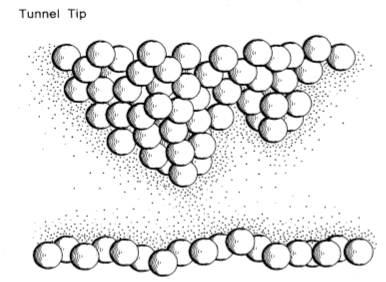
\includegraphics[width=0.47\textwidth]{pics/multitip}
  \end{center}
\caption{Schematische Abbildung aus \cite{binnig1987scanning}
mit strukturelle Aufbau der Spitze.} 
  \vspace{+20pt}
 \label{fig:multitip}

\end{wrapfigure}
Die erste Anwendung, welche die RTMs bekannt
machte, war die Oberflächenrekonstruktion von Silizium(111)  
\cite{binnig19837} (siehe Abbildung~\ref{fig:silicium}).
Dabei handelte es sich um ein offenes Problem in der
Festkörperphysik. Wie sich später durch die experimentelle
Aufarbeitung zeigte, waren die theoretischen Vorhersagen nicht 
korrekt und mussten korrigiert werden, gerade auch deswegen
erlangte die Rastertunnelmikroskopie ab 1985 große Bekannheit.
\begin{SCfigure}

\centering
\caption{Erste Anwendung des Rastertunnelmikroskops 
\cite{binnig19837}: 
Oberflächenrekonstruktion von Silizium(111) (siehe Millersche
Indizes im Theorieteil), welches eine komplexe (7x7) 
Überstrukturzelle besitzt}

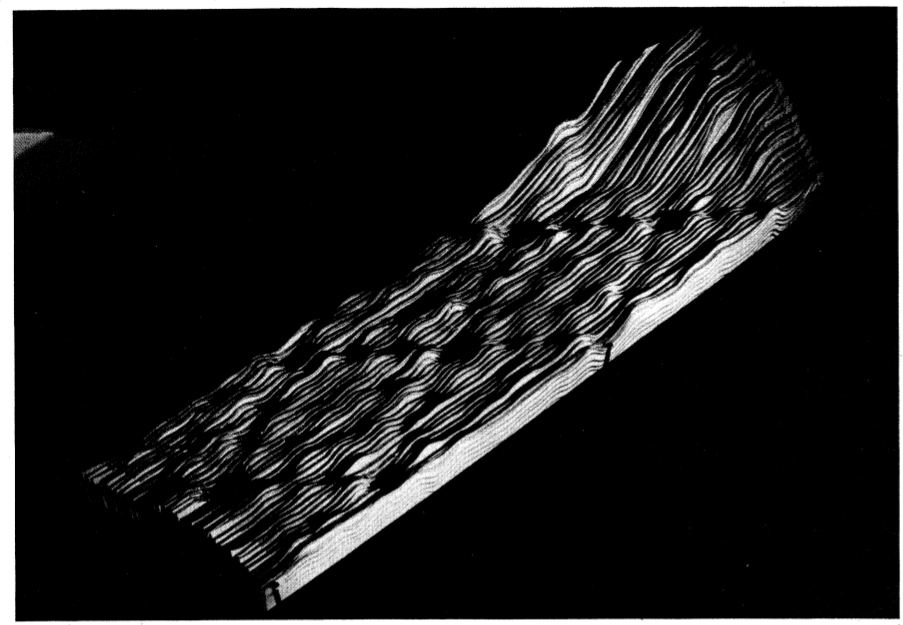
\includegraphics[width=0.48\textwidth]{pics/silicium}
 \label{fig:silicium}
\end{SCfigure}
Auf ihr baut die gesamte Rastersondenmikroskopie auf, welche
in einigen Spielarten in der Zeit danach weiterentwickelt wurde.
So war ist mit dem \textit{Rasterkraftmikroskop}
und dem \textit{optische Rasternahfeldmikroskop} möglich, sogar
nichtleitende Proben zu untersuchen, da das Abrastern nicht auf
einen geschlossenen Stromkreis basiert, sondern auf Kräften 
atomarer Ebene (Coulomb, Pauliprinzip). Somit bilden sie die Basis
für viele Anwendungen in der Chemie und Biologie.\\
1993 gelang es M.F. Crommie, C.P.Lutz und
D.M Eigler \cite{crommie1993imaging} dann
ein sogenanntes \textit{Quantengehege} aufzubauen
        (engl. \textit{Quantum Corral}), also eine Anzahl
von Atomen, welche auf einem Substrat ringförmig angeordnet sind.
Diese interferieren innerhalb des Ringes miteinander, sodass 
eine stehende Welle entsteht. Diese Quantum Corrals wurden 
wegen ihrer Anschaulichkeit der ihrer zugrunde liegenden
Quantenmechanik sehr populär, somit konnten mithilfe
des RTMs sogar Interferenzphänomene von Atomen
sichtbar gemacht werden (siehe Abbildung~\ref{fig:quantum_corral}). 

\begin{SCfigure}
\centering
\caption{Die Abbildung zeigt die 
    Visualisierung des Quantumgeheges, welches 1993 von 
    Crommie, Lutz und Eigler mithilfe des RTMs 
    konstruiert werden konnte \cite{crommie1993imaging}. 
    Speziell in dieser Abbildung ist eine 48-Eisen-atomige 
Ring konstruktion zu sehen, welche auf Kupfer(111) aufgebaut wurde.
Der Durchschnittsdurchmesser des Rings beträgt 142.6\r{A}.}
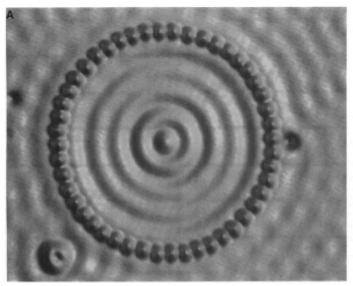
\includegraphics[width=7cm]{pics/quantum_corral}
 \label{fig:quantum_corral}
\end{SCfigure}

